%!TEX program = xelatex
\documentclass{article}
\usepackage[a5paper,hmargin=17mm,tmargin=15mm,bmargin=25mm]{geometry}

\usepackage{ifxetex}
\ifxetex
 \usepackage{fontspec}
 \setmainfont[Scale=1.1]{Arno Pro}
 \setmonofont[Scale=.92]{Consolas}
 \usepackage{unicode-math}              %% пакет для загрузки шрифтов математического режима 
 \setmathfont{[latinmodern-math.otf]}
 \setmathfont[range=\mathit/{latin,Latin}]{Arno Pro Italic}
 \setmathfont[range=up]{Arno Pro}
 \setmathfont[range=\mathup/{latin,Latin}]{Arno Pro}
\else
 \usepackage[utf8]{inputenc}
\fi
\usepackage[russian]{babel}
\usepackage{enumitem, graphicx, minted, microtype}
\usepackage[dvipsnames]{xcolor}

\newcommand{\textex}[1]{\texttt{\color{ForestGreen}#1}}


\begin{document}
\noindent
\textbf{Лабораторная работа 7}\\
{\Large \textbf{Функции. Рекурсия.}}\\
\strut\hfill\smash{\includegraphics[scale=0.2]{logo.png}}

Цель этой лабораторной работы~--- изучить понятие функции в языках Си и Си++ и научиться объявлять, определять и вызывать функции.

Функции~--- инструмент для управления сложностью. С помощь функций можно разделять программу на более удобные осмысленные части, избегать повторения кода, скрывать подробности низкого уровня. Функцию можно сравнить с мини-программой, которая имеет имя и решает определенную задачу. Чтобы ею пользоваться, вам не надо знать, как она устроена, достаточно знать, как она называется, как ей передать данные и как получить результат.

Например, если вы пишете программу для рисования графика температуры за год, можно написать функцию \texttt{getTemp(date)}, которая возвращает в виде числа температуру за указанную дату с одного из публичных серверов исторических погодных данных. После этого вы сможете вызывать ее для каждого из дней года и заняться вопросами красивого отображения графика, не волнуясь об адресе сервера, формате запроса, преобразовании ответа в число и тому подобных деталях.

Другой пример. Вот как могла бы выглядеть функция, которая находит длину строки:
\begin{minted}{cpp}
    int strlen(char* s) {
        int i = 0;
        while (s[i]!='\0')
            i++;
        return i;
    }
\end{minted}
Это \emph{определение} функции. В общем случае определение выглядит так:
\begin{verbatim}
    <тип> <имя функции>(<имена и типы параметров>) {
        <тело функции>
    }
\end{verbatim}
Тело функции должно содержать оператор \texttt{return}, который завершает ее выполнение, \emph{возвращая} в точку вызова некоторое значение указанного типа. Единственное исключение~--- функции, которые ничего не возвращают, а просто выполняют какие-то действия. Такие функции часто называют \emph{процедурами}, и для их объявления используется тип \texttt{void}.

\emph{Параметры} можно воспринимать как локальные переменные, которые при вызове функции автоматически получают значения переданных в нее аргументов.

Рассмотрим пример:
\begin{minted}{cpp}
  // main.cpp: один из корней квадратного уравнения 2x^2+3x-9=0
  #include <iostream>
  #include <cmath>
  double x1(double a, double b, double c) {
      double D = b*b - 4*a*c;
      return (-b - sqrt(D))/(2*a);
  }
  int main(){
      std::cout << x1(2, 3, -9) + 2;
  }
\end{minted}

Поскольку оператор \texttt{+} имеет более высокий приоритет, чем \texttt{<<}, сперва вычисляется значение суммы, а для этого должно быть сначала вычислено значение ее первого слагаемого: функция \texttt{main} приостанавливается и вызывает функцию \texttt{x1}. Это мини-программа, в ней есть собственная переменная \texttt{D}, а~также переменные-параметры \texttt{a}, \texttt{b}, \texttt{c}, причем выполнение функции невидимо начинается с присваиваний \texttt{a=2; b=3; c=-9;} для этих <<как бы>> переменных. Вычисленное значение корня уравнения, \texttt{-3}, возвращается в \texttt{main}, которая продолжает свое исполнение, заменяя \texttt{x1(2, 3, -9)} полученным от нее значением \texttt{-3}. Итак, в выходной поток выводится вычисленное значение суммы $-3 + 2 = -1$.

Для локальных переменных, то есть переменных, определенных внутри функции, применяется обычное правило: переменная видна только в ближайшем окружающем блоке, или фигурных скобках. В примере выше переменная \texttt{D} видна только внутри функции \texttt{x1} и недоступна из \texttt{main}. В разных функциях могут быть переменные с~одинаковыми именами, но внутри каждой из функций это имя будет означать свою переменную.

Функции \texttt{main}, для того чтобы вызвать \texttt{x1}, ничего не надо знать о том, как она устроена. Надо лишь остановиться в месте вызова, запустить функцию \texttt{x1}, передать ей три \texttt{double}-числа  и получить от нее одно число в~ответ. Поэтому для компиляции файла \texttt{main.cpp} достаточно на самом деле лишь \emph{определения}:
\begin{minted}{cpp}
   double x1(double a, double b, double c);
\end{minted}
Оно сообщает всю необходимую информацию для вызова и возврата значения, но не содержит тела функции. Другое отличие объявления от определения в том, что одинаковых объявлений может быть много, а определение~--- только одно.

Разберем подробнее процесс построения исходного файла. Именно для организации этого процесса нужны проекты и решения в Visual Studio. 

Хотя сборка в современной среде разработки обычно запускается одной кнопкой и может выглядеть как одно действие, в действительности процесс сборки состоит из нескольких этапов:
\begin{itemize}[nolistsep]
    \item[--] 
    препроцессинга, 
    \item[--]
    компиляции, 
    \item[--]
    компоновки. 
\end{itemize}

В ходе \emph{компиляции} файлы исходного кода на языке программирования преобразуются в объектные модули, состоящие из машинного кода. Для компиляции одного файла все используемые в нем функции должны быть объявлены, но не обязательно определены. В места вызова еще не определенных функций в объектные модули вставляются заглушки. 

Вы могли заметить, что мы не копировали объявления функций \texttt{scanf} / \texttt{printf} в код наших программ.  Часто функции собираются \emph{в библиотеку}, которая охватывает определенную область, например, как раз стандартный ввод-вывод. Было бы неудобно каждый раз выбирать и вставлять в каждый файл объявления используемых функций. Поэтому объявления всех функций, реализуемых библиотекой, собираются ее разработчиками в один общий заголовочный файл. И \texttt{stdio.h} представляет собой именно заголовочный файл. Чтобы не копипастить объявления, придумали \texttt{\#include}. Все директивы, начинающиеся с решетки, обрабатываются на этапе \emph{препроцессинга} (первый пункт в списке выше). Препроцессор просто заменяет \texttt{\#include <stdio.h>} на содержимое файла \texttt{stdio.h}, то есть в вашу программу вставляются все объявления еще до того, как она дойдет до этапа компиляции. 

Наконец, в ходе \emph{компоновки} код нескольких объектных модулей (и библиотек) собирается в один исполняемый файл, а все заглушки заменяются на реальные вызовы соответствующих функций. чтобы отслеживать все зависимости и собирать настройки компиляции в одном удобном месте, и придумали системы сборки, одной из которых является MSBuild, графический интерфейс к которому и есть система проектов и решений Visual Studio.

На рисунке ниже проиллюстрирован процесс сборки гипотетической сетевой игры, в которой по отдельным файлам (светло-зеленые) разделены основной геймплей (my.cpp), логика противников (enemy.cpp) и сетевой функциионал (net.cpp). Используемые заголовочные файлы изображены темно-зеленым цветом, голубым выделены объектные модули, синим~--- библиотечные модули, оранжевым~--- итоговый исполняемый файл приложения. 





\begin{figure}
\includegraphics[scale=0.5]{link.png}
\caption{Процесс сборки программы}
\end{figure}






\newpage
\begin{verse}
\small\it
У попа была собака,\\
Он ее любил.\\
Она съела кусок мяса,\\
Он ее убил.\\
В землю закопал, \\
Надпись написал, что:\\
У попа была собака\ldots
\end{verse}

Наверное вы догадались, к чему здесь этот жестокий стишок. Вы уже сталкивались с рекурсией при рассмотрении быстрой сортировки. В отличие от повтора или выбора действия, рекурсия редко встречается в повседневной жизни. Поэтому ею не так легко овладеть, однако такой способ мышления позволяет решать многие задачи, которые трудно с разбегу решить при помощи итерации. Поэтому навыки решения задач при помощи рекурсии~--- стоящее дополнение к вашему набору умений. 

Ключевой момент здесь --- умение выделить в задаче меньшую задачу такого же типа. Иногда упоминают метафору <<сделать наименьшее количество работы, чтобы тебя нельзя было назвать бездельником, и спустить остальное подчиненным>>. Иногда наоборот, удобнее смотреть на задачу, предполагая, что любую меньшую задачу мы уже умеем решать. В любом случае в тексте программы рекурсия выглядит как вызов изнутри функции самой этой функции, но с другими, обычно меньшими, параметрами. Поскольку такая цепочка вызовов продолжаться бесконечно не может (даже у самого большого начальника нет бесконечного числа подчиненных, поп писать устанет), какой-то самый простой случай задачи должен решаться без рекурсивного вызова.

Рассмотрим пример. Нужно найти сумму целочисленного массива размера $N$, написав функцию \texttt{int sum(int* A, unsigned N)}. Для интереса попробуем придумать рекурсивное решение. Представим, что нам лень выполнять сложение больше одного раза. Сумму какого массива мы можем найти вообще без сложения? Массива размера 1. Теперь предположим, что мы уже умеем решать все меньшие задачи, то есть у нас есть помощник \texttt{sum(...)}. Заставим его просуммировать все $N-1$ элементов массива, оставив себе лишь последний. Когда он вычислит почти всю сумму, прибавим к ней последний элемент и присвоим все лавры себе. Получилось рекурсивное решение:
\begin{minted}{cpp}
int sum(int* A, unsigned N){
    if (N==1)
        return A[0];
    else
        return sum(A, N-1) + A[N-1];
}
\end{minted}






\newpage
\begin{center}
\textbf{ОБЩИЕ ЗАДАНИЯ}
\end{center}

\sloppy
\begin{enumerate}
\item
Напишите функцию возведения вещественного числа в целую неотрицательную степень \texttt{double power(double x, unsigned k)}, которая вычисляет $x^k$. Напишите с ее помощью программу, которая вводит целое значение показателя степени $m$, и выводит через пробел $m$-ые степени чисел 1, 2, \ldots, 10. Заголовочные файлы \texttt{math.h/cmath} не использовать.

Пример ввода: \textex{2}, правильный вывод \textex{1 4 9 16 25 36 49 64 81 100}.

\item
Напишите функцию \texttt{double dist(x1, y1, x2, y2)}, которая принимает вещественные декартовы координаты двух точек на плоскости и возвращает расстояние между ними. Напишите с ее помощью программу, которая вводит вещественные координаты $x_1$, $y_1$, $x_2$, $y_2$, $x_3$, $y_3$ трех точек на плоскости и выводит длину самой длинной стороны треугольника с вершинами в этих точках, или –1, если такого треугольника не существует.

Пример ввода: \textex{0 0 6 0 3 2}, правильный вывод \textex{6}.

\item
Напишите функцию \texttt{unsigned word\_end(char* s, unsigned i)}, 
которая принимает строку $s$, состоящую из одних латинских букв и пробелов, и индекс $i$ в ней ($0 \leqslant i<\mbox{\texttt{strlen}}(s)$). Функция должна возвращать индекс символа, следующего за последним символом слова, которому принадлежит символ $s[i]$. Напишите с помощью этой функции программу, которая вводит число $k$, затем строку, состоящую из одних латинских букв и пробелов, и выводит $k$-е слово строки (считая с 1).

Примеры. Для строки $s={}$\verb!"!\texttt{This is fine"}
значение \texttt{word\_end(s, 0)}  равно 4,  значение \texttt{word\_end(s, 9)} равно 12.
Для $k=3$ с таким $s$ программа должна ответить \textex{fine}.

\item
Напишите рекурсивный вариант вычисления минимума целочисленного массива в виде функции \texttt{int min(int* A, unsigned n)}, находящей минимум среди первых $n$ элементов массива $A$. Напишите с помощью этой функции программу, которая вводит число $N$, динамически создает массив размера $N$, заполняет его с клавиатуры и выводит минимум массива.

\item
Напишите рекурсивный вариант функции, определеющей, является ли подстрока строки $s$, начиающаяся в $i$-м и завершающаяся \underline{перед} $j$-м символом, палиндромом. Функция должна быть реализована как \texttt{bool isPalindrome(char* s, unsigned i, unsigned j)}. Напишите с помощью этой функции программу, которая вводит строку $s$, длины не превышающей 100, и отвечает на вопрос, является ли она палиндромом. Символы считать одинаковыми только при точном совпадении ($\texttt{'a'}\ne\texttt{'A'}$), пробелы не игнорировать.

\end{enumerate}









\bigskip\sloppy

\noindent\centerline{\textbf{ИНДИВИДУАЛЬНЫЕ ЗАДАНИЯ}}

\medskip
\textbf{
Всего в этом домашнем задании 3 пункта. Из каждого пункта надо сделать по одной задаче, в зависимости от вашего номера в списке группы. Считать по кругу: если в пункте 5 задач, то 6-й номер делает первую задачу, 7-й номер вторую и т.\,д.}

\textbf{Проверять корректность ввода, например, что треугольник со введенными сторонами действительно существует, не надо. Обратите внимание: обратные тригонометрические функции из \texttt{<math.h>} типа арккосинуса (\texttt{acos}) возвращают значения углов в радианах. 
}

\begin{enumerate}[label={}, leftmargin=0pt, itemindent=0pt]

\item

\begin{enumerate}[label=\arabic{enumi}.\arabic*.] % ------- #1 -------
\item
Напишите функцию \texttt{sumsq(a,b,c)}, возвращающую сумму квадратов трех вещественных чисел $a$, $b$, $c$. Напишите с использованием этой функции программу, которая вводит натуральное число $n\geqslant 3$, затем $n$ вещественных чисел $x_0, x_1, \ldots x_{n-1}$, и выводит максимальную сумму квадратов для трех соседних элементов последовательности $\{x_i\}$.

\noindent Пример ввода: \\
\textex{4\\
1 -1.4142 2 0}\\
Правильный вывод: \textex{7}

\item
Напишите функцию \texttt{diff(a,b,c)}, возвращающую разность между максимум и минимумом трех целых чисел $a$, $b$, $c$. Напишите с использованием этой функции программу, которая вводит натуральное число $n\geqslant 3$, затем $n$ вещественных чисел $x_0, x_1, \ldots x_{n-1}$, и выводит три соседних элемента последовательности $\{x_i\}$с минимальным значением функции \texttt{diff}.

\noindent Пример ввода: \\
\textex{4\\
1 5 6 9}\\
Правильный вывод: \textex{5 6 9}

\item
Напишите функцию \texttt{sumabs(a,b,c)}, возвращающую сумму модулей трех вещественных чисел $a$, $b$, $c$. Напишите с использованием этой функции программу, которая вводит натуральное число $n\geqslant 3$, затем $n$ вещественных чисел, и выводит три соседних числа среди них, имеющие максимальную сумму модулей:

\noindent Пример ввода: \\
\textex{5\\
1 -1.4142 2 0 1}\\
Правильный вывод: \textex{1 -1.4142 2}

\item
Напишите функцию \texttt{factorial(n)}, возвращающую факториал целоко неотрицательного числа $n$. Напишите с использованием этой функции программу, которая вводит неотрицательные целые числа $n$ , $k$  ($k\leqslant n$), и выводит значение числа сочетаний по $k$из $n$ элементов: $$C_n^k = \frac{n!}{k!(n-k)!}$$

\noindent Пример ввода: \textex{5 3}\\
Правильный вывод: \textex{10}

\item
Напишите функцию \texttt{gcd(a,b)} нахождения наибольшего общего делителя двух неотрицательных целых чисел по алгоритму Евклида. Алгоритм Евклида: вычитать из максимального числа пары другое, пока одно из чисел не станет нулем, тогда другое число и есть НОД. При помощи этой функции напишите функцию \texttt{gcd3(a,b,c)}, находящую наибольший общий делитель трех чисел, и программу, которая вводит три неотрицательных целых числа $a$, $b$, $c$ и выводит значение \texttt{gcd3(a,b,c)}.

\noindent Пример ввода: \textex{24 72 14}\\
Правильный вывод: \textex{2}
\end{enumerate}

\medskip\hrulefill\medskip
\item 

\begin{enumerate}[label=\arabic{enumi}.\arabic*.] % ------- 2 -------
\item
Напишите функцию \texttt{angle(x,y,z)}, которая дает угол, противолежащий стороне $z$ в треугольнике со сторонами $x$, $y$, $z$. Напишите с использованием этой функции программу, которая вводит вещественные длины трех сторон треугольника и выводит углы, противолежащие сторонам в том же порядке, в градусах c фиксированной точностью 1 знак после десятичной точки.

\noindent
Пример ввода: \textex{1 1 1.4142}\\
Правильный вывод: \textex{45.0 45.0 90.0}

\item
Напишите функцию \texttt{angle(x1,y1,x2,y2,x3,y3)}, которая принимает целые координаты точек $A(x_1, y_1)$, $B(x_2, y_2)$, $C(x_3, y_3)$ и дает тот угол между отрезками $AB$ и $BC$, который не больше $\pi$, в радианах. Напишите с использованием этой функции программу, которая вводит число $n$, затем $2n$ целых чисел~--- координаты вершин ломаной в виде $x_0, y_0, x_1, y_1, \ldots$, и выводит максимальный угол во внутренней вершине ломаной с четырьмя знаками после десятичной точки.

\noindent
Пример ввода: \\
\textex{5\\
2 0 1 1 2 1 2 2 3 1}\\
Правильный вывод: \textex{1.5708}

\vskip-1.7cm\strut\hfill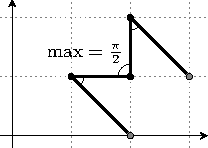
\includegraphics{segments.pdf}

\item
Напишите функцию \texttt{visibleAngle(x1,y1,x2,y2,x,y)}, которая определяет, под каким углом отрезок $AB$ виден из точки $C$ вне него, если координаты точек имеют вид $A(x_1, y_1)$, $B(x_2,y_2)$, $C(x,y)$. Напишите с использованием этой функции программу, которая вводит число $n$, затем $2n$ целых чисел~--- координаты вершин ломаной в виде $x_0, y_0, x_1, y_1,\ldots$, и выводит максимальный угол, под которым из какой-либо вершины ломаной $(x_i,y_i)$ виден ее следующий отрезок $(x_{i+1},y_{i+1})-(x_{i+2},y_{i+2})$, в~радианах с четырьмя знаками после десятичной точки.

\noindent
Пример ввода: \\
\textex{5\\
0 0 1 1 2 1 2 2 3 1}\\
Правильный вывод: \textex{1.5708}

\vskip-1.7cm\strut\hfill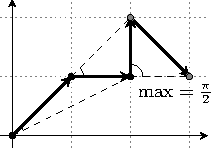
\includegraphics{maxview.pdf}
\end{enumerate}


\medskip\hrulefill\medskip

\item 

\begin{enumerate}[label=\arabic{enumi}.\arabic*.] % ------- 3 -------
\item
Напишите рекурсивную функцию \texttt{reverse(n)}, которая возвращает число с обратным порядком цифр относительно $n$. Если обращение $n$ приводит к ведущим нулям, они игнорируются, например \texttt{reverse(\textex{1900})} равно \textex{91}. Напишите с использованием этой функции программу, которая вводит число $n$ и выводит его обращение.

\noindent Пример ввода: \textex{7405}, правильный вывод: \textex{5047}.
\item
Напишите рекурсивную функцию \texttt{reverse(s, n)}, которая принимает строку \texttt{s} длины \texttt{n} и выводит на экран ее символы в обратном порядке. Функция ничего не возвращает, строку \texttt{s} не изменяет. Напишите с использованием этой функции программу, которая вводит строку и выводит ее обращение.

\noindent Пример ввода: \textex{alpha}, правильный вывод: \textex{ahpla}.

\item
Напишите рекурсивную функцию \texttt{indexOf(A,i,j,x)}, которая ищет в элементах \texttt{A[i]}, \texttt{A[i+1]}, \ldots \texttt{A[j-1]} неупорядоченного целочисленного массива \texttt{A} число \texttt{x} и возвращает либо индекс первого вхождения \texttt{x} в указанный отрезок массива, либо \texttt{-1}, если \texttt{x} в нем не встречается. Напишите с использованием этой функции программу, которая вводит натуральное число $n\geqslant 3$, затем $n$ целых чисел $A_0, A_1, \ldots A_{n-1}$, затем число $x$ и выводит значение функции \texttt{indexOf(A,0,n,x)}.

\noindent Пример ввода: \\
\textex{5\\4 2 3 8 1\\3}
\\
Правильный вывод: \textex{2}.

\item
Напишите рекурсивную функцию 
\begin{minted}{cpp}
    long long decimal(long long x)
\end{minted}
которая принимает длинное неотрицательное целое число $x$ и, рассматривая его цифры как восьмеричную запись, возвращает его десятичное представление. Напишите с использованием этой функции программу, которая вводит восьмеричное натуральное число $n\geqslant 3$ в переменную типа \texttt{long long} и выводит его десятичную запись. Гарантируется, что во введенном числе нет цифр 8, 9.

\noindent Пример ввода: \textex{123}, правильный вывод: \textex{83}.
\end{enumerate}

\end{enumerate}




\end{document}
